\synctex=1
\documentclass[dvipdfmx,10pt, a4j]{jarticle}
%----------------------------------------------------------
%パッケージ読み込み
\usepackage{amsmath}
\usepackage{amssymb}
\usepackage{amsthm} %定理環境の拡張
\usepackage{ascmac}
\usepackage{bm}
\usepackage{cases}
\usepackage{comment} %非表示にするためのコメント
\usepackage{enumerate}
\usepackage{float} %画像をその場に表示.[h]の代わりに[H]
\usepackage{graphicx} % eps 形式の図版取り込みのため
% \usepackage[dviout]{graphicx}
\usepackage{mathrsfs}
\usepackage{url}
\usepackage[dvipdfmx]{hyperref}
\usepackage{color}
%----------------------------------------------------------

%----------------------------------------------------------
%命題関係の定義
\theoremstyle{definition}
\newtheorem{definition}{定義}[section]
\newtheorem{theorem}{定理}[section]
\newtheorem{proposition}[theorem]{命題}
\newtheorem{lemma}[theorem]{補題}
\newtheorem{col}[theorem]{系}
\newtheorem{example}{例}[section]
\newtheorem{remark}{注意}[section]
%----------------------------------------------------------

%タイトル・著者===================================================
\title{第6回 数理統計 レポート}
\author{小森 一輝}
%=================================================================

%本文開始=========================================================
\begin{document}

\maketitle

%カウンタ--------------------------------------------------
\setcounter{section}{2}
%\setcounter{subsection}{0}
%\setcounter{subsubsection}{0}
%\setcounter{theorem}{0}

    %----------------------------------------------------------定義3.2
    \noindent
    \textbf{定義 3.2.} 可測関数, ボレル関数\\
    $可測空間(\Omega_1, \mathcal{A}_1) から, 可測空間(\Omega, \mathcal{A}_2)への写像T : \Omega_1 \to \Omega_2が,$\\
    \begin{align*}
        T^{-1}(B) \in \mathcal{A}_1 \qquad (B \in \mathcal{A}_2)
    \end{align*}
    $を満たすとき, Tは(\mathcal{A}_1, \mathcal{A}_2) 上の \textbf{可測な写像}であるという。$
    $特に, (\Omega_2, \mathcal{A}_2) = (\mathbb{R}, \mathcal{B})のとき, Tを(\Omega_1, \mathcal{A}_1)上の \textbf{可測関数} という。$
    $また, (\Omega_1, \mathcal{A}_1) = (\Omega_2, \mathcal{A}_2) = (\mathbb{R}, \mathcal{B}) のとき, Tを \textbf{ボレル関数} という。$\\

    %----------------------------------------------------------定理3.4
    \noindent
    \textbf{定理 3.4.} $Xを (\Omega, \mathcal{A}, P)上の確率変数とし, 関数h: \mathbb{R} \to \mathbb{R} とする.$\\
    
    %----------------------------------------------------------定理3.5
    \noindent
    \textbf{定理 3.5.} $確率空間 (\Omega, \mathcal{A}, P) における, 確率変数 X に対して,$\\
    \begin{align*}
        &P_X(B) = P(X^{-1}(B)) \qquad (B \in \mathcal{B})\\
        &(\mathcal{B} : ボレルセット, B: 区間, P(X^{-1}(B)): 確率)\\
    \end{align*}
    $によって, (\mathbb{R}, \mathcal{B})上の確率速度 P_Xが定義され, 確率空間 (\mathbb{R}, \mathcal{B}, P_X) が導かれる.$\\
    $P_Xが確率空間であることを示す.$
    \begin{proof} $P_X が確率になることを示す.$\\
        \begin{enumerate}[i)]
            \item $0 \leq P_X(B) = P(X^{-1}(B)) \leq 1 が成り立つ.$\\
            \item $P_X(\mathbb{R}) = P(X^{-1}(\mathbb{R})) = P(\Omega) = 1 となり, 成り立つ. \qquad (P(\Omega) = 1)$\\
            \item $B_i \in B (i = 1, 2, \dots), B_i \cap B_j = \phi (i \neq j)$\\
            \begin{align*}
                &P_X(\bigcup_{i=1}^{\infty}{B_i}) = P(X^{-1}(\bigcup_{i=1}^{\infty}{B_i})) = P(\bigcup_{i=1}^{\infty}{X^{-1}(B_i)}) \quad (\because 逆像)\\
                &= \sum_{i=1}^{\infty}{P(X^{-1}(B_i))} = \sum_{i=1}^{\infty}{P_X(B_i)}\\
                &となり, 成り立つ.
            \end{align*}
        \end{enumerate}
    \end{proof}
    
    %----------------------------------------------------------定義3.3
    \noindent
    \textbf{定義 3.3.} 確率分布\\
    $定理3.5によって定義された(\mathbb{R}, \mathcal{B})上の確率測度 P_X は確率変数 X の\textbf{確率分布} と呼ばれる.$
    $このとき, X は確率分布 P_X に従うといい, X ~ P_Xと記す.$\\
    
    %----------------------------------------------------------定義3.4
    \noindent
    \textbf{定義 3.4.} 分布関数\\
    $確率空間 (\Omega, \mathcal{A}, P) における確率変数 X に対して,$\\
    \begin{align*}
        F_X(x) = P_X((- \infty, x]) = P(\{ \omega \mid X(\omega) \leq x \}) \qquad (x \in \mathbb{R})\\
    \end{align*}
    $で定義される \mathbb{R} 上の実数値関数 F_X を X の \textbf{分布関数} とよぶ.$\\
    %---------------以下補足
    \begin{itembox}[l]{補足}
        \begin{align*}
            &確率 &P(\{ \omega \mid X(\omega) \leq x \}) \quad (事象) \quad (x \in \mathbb{R})\\
            &確率分布 &= P_X((- \infty, x]) \quad (区間)\\
            &分布関数 &= F_X(x) \quad (実数)\\
        \end{align*}
    \end{itembox}\\
    
    %----------------------------------------------------------定理3.6
    \noindent
    \textbf{定理 3.6.} 分布関数の性質\\
    $確率変数X の分布関数F_X は次の性質を満たす.$\\
    \begin{enumerate}[i)]
        \item $F_X は単調非減少である.すなわち, x < y \rightarrow F_X(x) \leq F_Y(y) である.$\\
        \item $F_X は右連続である. すなわち, \displaystyle \lim_{y \to x+0}F_X(y) = F_X(x)である.$\\
        \item $F_X (- \infty) = \displaystyle \lim_{x \to - \infty}F_X(x) = 0, \quad F_X(\infty) = \displaystyle \lim_{x \to \infty}F_X(x) = 1 である. \quad (階段関数もOK)$\\
    \end{enumerate}
    \begin{figure}[htbp]
        \begin{center}
            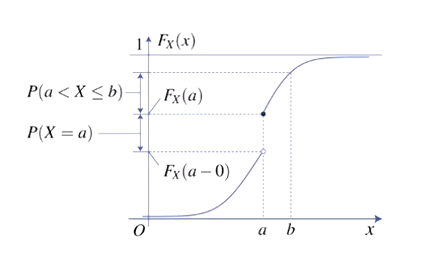
\includegraphics[width=7.0cm]{D_6/img_2.png}
            \caption{分布関数}
        \end{center}
    \end{figure}
    
    %----------------------------------------------------------定義3.5
    \newpage
    \noindent
    \textbf{定義 3.5.} 離散型確率変数\\
    $確率空間 (\Omega, \mathcal{A}, P) における確率変数 X に対して, 有限または可算無限集合 E = \{x_i \mid i = 1, 2, \dots\} が存在して,$
    $P(X \in E) = 1 を満たすとき, X を \textbf{離散型確率変数} とよぶ.$\\
    $以下, X が離散型確率変数であるとき, x_i \in E (i = 1, 2, \dots) に対して, $\\
    $p_i = P_X(\{x_i\}) = P(\{\omega \mid X(\omega) = x_i\})と定める. このとき,$\\
    \begin{align*}
        \sum_{i=1}^{\infty}{p_i} = 1, \qquad F_X(x) = \sum_{x_i < x}{p_i}\\
    \end{align*}
    が成り立つ.\\
    %---------------以下補足
    \begin{itembox}[l]{補足}
        \begin{align*}
            P_i = P_X(\{x_i\}) \quad (区間 (一点)) = P(\{\omega \mid X(\omega) = x_i\}) \quad (事象)\\
        \end{align*}
    \end{itembox}\\
    
    %----------------------------------------------------------定義3.6
    \newpage
    \noindent
    \textbf{定義 3.6.} 確率関数\\
    $\textcolor{red}{離散型確率変数 X} に対して, \mathbb{R} 上の実数値関数 f_X を$\\
    \begin{align*}
        f_X(x) =
        \begin{cases}
            p_i = P(\{x_i\}) \qquad (x = x_i \in E (i = 1, 2, \dots))\\
            0 \qquad (x \notin E)\\
        \end{cases}
    \end{align*}
    $で定義する(\textcolor{red}{定義域を \mathbb{R} にするため})とき, f_X を X の \textbf{確率関数} とよぶ.$\\
    %---------------以下図
    \begin{figure}[htbp]
        \begin{center}
            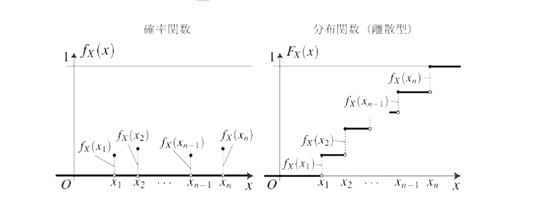
\includegraphics[width=14.0cm]{D_6/img_3.png}
            \caption{確率関数と分布関数(離散型)}
        \end{center}
    \end{figure}
    %---------------以下補足
    \begin{itembox}[l]{例 (サイコロ)}
        $E = \{1, 2, 3, 4, 5, 6\}$\\
        \begin{align*}
            f_X(x) =
            \begin{cases}
                \frac{1}{6} \quad (x = 1, 2, 3, 4, 5, 6)\\
                0 \quad (other)\\
            \end{cases}
        \end{align*}
    \end{itembox}\\
    
    %----------------------------------------------------------命題3.9
    \noindent
    \textbf{命題 3.9.} 確率関数の性質\\
    $離散型確率変数 X に対する 確率変数 f_X は次の性質をもつ.$\\
    \begin{align*}
        f_X(x) > 0, \qquad \sum_{i=1}^{\infty}f_X(x_i) = 1, \qquad F_X(x) = \sum_{x_i \leq x}f_X(x_i)\\
    \end{align*}
    
    %----------------------------------------------------------命題3.10
    \noindent
    \textbf{命題 3.10.} $離散型確率変数 X に対して, 以下が成り立つ.$\\
    \begin{align*}
        &P(X = x_i) = f_X(x_i) \quad (離散型の特徴)\\
        &P(a < x \leq b) = \sum_{a < x_i \leq b}{f_X(x)} \quad (区間の確率は和で書ける)\\
    \end{align*}
    
    %----------------------------------------------------------定義3.7
    \noindent
    \textbf{定義 3.7.} 連続型確率変数, 確率密度関数\\
    $確率空間 (\Omega, \mathcal{A}, P) における確率変数 X に対して, \mathbb{R} 上の非負値関数 f_X が存在し, 確率分布 P_Xが,$\\
    \begin{align*}
        P_X(B) = \int_{B}{f_X(x)}dx \qquad (B \in \mathcal{B})\\
    \end{align*}
    $によって表されるとき, f_X は X の \textbf{連続型確率変数} とよばれ, f_X は X の \textbf{確率密度関数} とよばれる.$\\
    %---------------以下図
    \begin{figure}[htbp]
        \begin{center}
            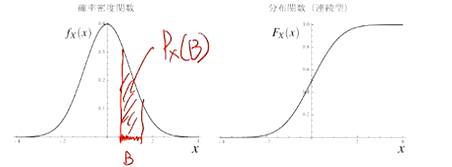
\includegraphics[width=7.0cm]{D_6/img_4.png}
            \caption{確率関数と分布関数(連続型)}
        \end{center}
    \end{figure}
    
    %----------------------------------------------------------命題3.11
    \noindent
    \textbf{命題 3.11.} 確率密度関数の性質\\
    $連続型確率変数 X に対する確率密度関数 f_X は次の性質を持つ.$\\
    \begin{align*}
        f_X(x) > 0 \quad (x \in \mathcal{R}), \qquad \int_{- \infty}^{\infty}{f_X(x)} = 1\\ 
    \end{align*}
    
    %----------------------------------------------------------命題3.12
    \noindent
    \textbf{命題 3.12.} 連続型確率変数 X について以下が成り立つ.\\
    \begin{align*}
        P(X = x) = 0 \qquad (x \in \mathcal{R})\\
        P(a < X \leq b) = \int_{a}^{b}{f_X(t)dt}\\
    \end{align*}
    
    %----------------------------------------------------------命題3.13
    \noindent
    \textbf{命題 3.13.} 確率変数の関数の分布関数\\
    $確率変数X のボレル関数h: \mathbb{R} \to \mathbb{R} による変数変換 Y = h(X)の分布関数 F_Y は次式で与えられる.$\\
    \begin{align*}
        F_Y(y) =
        \begin{cases}
            \sum_{x_i \in h^{-1}((- \infty, y])}{f_X(x_i)} \qquad (X が離散型)\\
            \int_{h^{-1}((- \infty, y])}{f_X(x)dx} \qquad (X が連続型)\\
        \end{cases}
    \end{align*}
    
    %----------------------------------------------------------命題3.14
    \noindent
    \textbf{命題 3.14.} 確率変数の関数の確率密度関数\\
    $連続型確率変数X のボレル関数h: \mathbb{R} \to \mathbb{R} による変数変換 Y = h(X)の分布関数 F_Y は$
    $\mathbb{R} において微分可能であり, かつ, その導関数 dF_Y/f_y が \mathbb{R} において積分可能であれば, 確率変数Y の確率密度関数は$\\
    \begin{align*}
        f_Y(y) = \frac{d}{dy}F_Y(y) \mid_{y=y} \qquad (y \in \mathbb{R})\\
    \end{align*}
    で与えられる.\\
    
    %----------------------------------------------------------定理3.15
    \noindent
    \textbf{定理 3.15.} $連続型確率変数 X が確率密度関数 f_X をもつとする. このとき, 以下が成り立つ$\\
    \begin{enumerate}[i)]
        \item $関数y = h(x) が区間 (a, b) で微分可能であり, かつ, 単調増加または単調減少であるとする.$
        $このとき, 確率変数Y = h(X) の確率密度関数は, 以下で与えられる.$\\
        \begin{align*}
            f_Y(y) = f_X(h^{-1}(y)) \mid \frac{d}{dy} h^{-1}(y) \mid \quad (\alpha < y < \beta)\\
        \end{align*}
        $ただし, \; \alpha = min(h(a), h(b)), \; \beta = max(h(a), h(b))である.$\\
        \item $関数y=h(x) を区分的に連続な確率変数h_i(x) で y = h_i(x) \; (x \in I_i) と分割する.$
        $ただし, I_i = (a_i, a_{i+1}] であり, I_i \cap I_j = \phi (i \neq j), \bigcup_{i=1}^{\infty}{I_i} = (a, b)とする.$
        $h_i を区間 I_i で微分可能であり, かつ, 単調減少であるとし, 区間 I_i での h_i の逆関数を h_i^{-1} で表す.$
        $このとき, y \in \bigcup_{i=1}^{\infty}{h_i}(I_i)を満たす y に対して, 確率変数 Y = h(X) の確率密度関数は, 以下で与えられる.$\\
        \begin{align*}
            f_Y(y) = \sum_{i =1}^{\infty}{f_X(h_i^{-1}(y)) \mid \frac{d}{dy} h_i^{-1}(y)} \mid\\
        \end{align*}
        
        %----------------------------------------------------------例3.2
        \noindent
        \textbf{例 3.2.} $Xを連続型確率変数とする. X の変数変換 Y = aX + b (a, b \in \mathbb{R}, a \neq 0)$
        $確率密度関数 f_Y は X の確率密度関数 f_X を用いて, 以下のように表される.$\\
        \begin{align*}
            f_Y(y) = \frac{1}{\mid a \mid}f_X \left(\frac{y-b}{a} \right)\\
        \end{align*}
        
        %----------------------------------------------------------例3.3
        \noindent
        \textbf{例 3.3.} $Xを連続型確率変数とする. X の変数変換 Y_1 = e^{X}, Y_2 = logX, Y_3 = |X|, Y_4 = X^{2} の確率密度関数 f_{Y_1}, f_{Y_2}, f_{Y_3}, f_{Y_4}$
        $はXの確率密度関数 f_X を用いて, 以下のように表される.$\\
        \begin{align*}
            &f_{Y_1}(y) = \frac{1}{y}f_X(logy) \qquad (y > 0)\\
            &f_{Y_2}(y) = e^{y}f_X(e^{y})\\
            &f_{Y_3}(y) =
            \begin{cases}
                f_X(y) + f_X(-y) \qquad (y \geq 0)\\
                0 \qquad (y < 0)\\
            \end{cases}\\
            &f_{Y_4}(y) =
            \begin{cases}
                \frac{1}{2 \sqrt{y}}(f_X(\sqrt{y}) + f_X(- \sqrt{y})) \qquad (y \geq 0)\\
                0 \qquad (y < 0)\\
            \end{cases}
        \end{align*}    
    \end{enumerate}
    \begin{enumerate}[(1)]
        \item $y = e^{x}$\\
        \begin{align*}
            &x = h^{-1}(y) = logy \quad (y > 0)\\
            &\frac{d}{dy}h^{-1}(y) = \frac{1}{y}\\
        \end{align*}
        \item $y \cdot logX \quad x = h^{-1}(y) = e^{y}, \quad \frac{d}{dy}h^{-1}(y) = e^{y}$\\
        \item $y = |x| \quad I_1 = (- \infty, 0], I_2 = (0, \infty]$\\
        $h, y, I_1で単調減少,I_2で単調増加$\\
        $y \geq 0 のとき,$\\
        \begin{align*}
            h^{-1}(y) =
            \begin{cases}
                -y \quad (x \in I_1)\\
                y \quad (x \in I_2)\\
            \end{cases}
        \end{align*}
        \begin{align*}
            \frac{d}{dy}h^{-1}(y) =
            \begin{cases}
                -1 \quad (x \in I_1)\\
                1 \quad (x \in I_2)\\
            \end{cases}
        \end{align*}
        \begin{align*}
            f_Y(y) + f_X(-y) =
            \begin{cases}
                f_X(y) \quad (y \geq 0)\\
                0 \quad (y < 0)\\
            \end{cases}
        \end{align*}
    \end{enumerate}
\end{document}
%本文ここまで=========================================================